\chapter{GloVe Model}\label{ch:glove}

%\section{Terminology}
%
%\begin{table}[!ht]
%  \begin{center}      
%      \begin{tabular}{l|c|m{6cm}}
%          \hline
%          \textbf{Notation} & \textbf{Symbol} & \parbox{6cm}{\centering\textbf{Description}} \\
%          \hline\hline
%          Vocabulary & $V$ & Set of unique words of the given corpus\\ \hline
%          Word vector & $w\ (w_i)$ & Word vector (of corresponding word $i$)\\ \hline
%          Context vector & $\tilde{w}\ (\tilde{w}_i)$ & Context vector (of corresponding word $i$)\\ \hline
%          Dimension   & $d$ & Dimension of word vectors $w$\\ \hline
%          Word-word co-occurence matrix & $X \in \mathbb{R}^{|V| \times |V|}$ & Matrix of context counts $X_{ij}$\\ \hline
%          Loss function & & \\ \hline
%          Empirical risk & & \\ \hline
%      \end{tabular}
%  \end{center}
%\caption{Overview about the used terminology.}
%\label{tab:terminology}
%\end{table}

\section{Word-Word Co-Occurence Matrix}

Base of the model is the word-word co-occurrence matrix 
$X \in \mathbb{R}^{|V| \times |V|}$, where $|V|$ is the number of different 
words which occurs within a given corpus. In $X$ every entry
$X_{ij}$ describes how often word $j$ occurs in context of word $i$ with a given
window size. Therefore we have the following properties:

\begin{itemize}
  \item $X_i = \sum_k X_{ik}$: Number of words which occur in the context of $i$.
  \item $P_{ij} = P(j | i) = X_{ij} / X_i$: "Probability" of word $j$ occurs in context of $i$.
  \item The ratio $P_{ik} / P_{jk}$ describes if word $k$ is more related to \dots
    \begin{itemize}
      \item \dots word $i$ if  $P_{ik} / P_{jk} > 1$
      \item \dots word $j$ if $P_{ik} / P_{jk} < 1$
      \item \dots or similar related if $P_{ik} / P_{jk} \approx 1$    
    \end{itemize}
\end{itemize}

\textbf{Example: word-word co-occurenece Matrix} \\

To understand how an entry of the word-word co-occurence matrix is computed we take a 
look at the following sample corpus:

\begin{center}
A D C E A D E B A C E D $\ \Rightarrow\ V = \{\text{A B C D E}\},\ |V| = 5$
\end{center}

Furthermore, we need to specify a window size which indicate how much words we want to look
at around a specific word. We choose a window size of 2 (the 2 words of the either side)  
for this example. With the given corpus and the window size we now compute the counts of
how often word D occurs in context of word A ($X_{AD}$):

\begin{center}
\textcolor{red}{A} \textcolor{orange}{D C} E A D E B A C E D $\ \Rightarrow$ D occurs 1 time \\
A D \textcolor{orange}{C E} \textcolor{red}{A} \textcolor{orange}{D E} B A C E D $\ \Rightarrow$ D occurs 1 time \\
A D C E A D \textcolor{orange}{E B} \textcolor{red}{A} \textcolor{orange}{C E} D $\ \Rightarrow$ D occurs 0 times \\
\phantom{A D C E A D E B A C E D} $\ \Rightarrow$ D occurs 2 times in context of A: $X_{AD} = 2$
\end{center}

Finally, we do this for every word combination of $(i, j) \in V \times V$ and calculate the 
ratio $P_{AD}$:

\begin{center}
$X = $
\begin{tabular}{c|ccccc}
         & \text{A} & \text{B} & \text{C} & \text{D} & \text{E} \\
\hline
\text{A} &     0    &     1    &     3    &     2    &     4  \\
\text{B} &     1    &     0    &     1    &     1    &     1  \\
\text{C} &     3    &     1    &     0    &     2    &     2  \\
\text{D} &     2    &     1    &     2    &     0    &     4  \\
\text{E} &     4    &     1    &     2    &     4    &     0
\end{tabular}$ \ \ \Rightarrow\ \ P_\text{AD} = X_\text{AD} / X_\text{A} = 2/10$
\end{center}


\textbf{Sidenote:} \\

Some packages (like \texttt{R}'s \texttt{text2vec}) have an option to give a weight vector
with as many weights as the window size. It is then common to weight context words closer to 
the inspected word higher than words which aren't that close.

\section{The Model}

GloVe was introduced by Jeffrey Pennington, Richard Socher and 
Christopher D.Manning \cite{pennington2014glove}: 

\begin{quote}
\enquote{\textit{... GloVe is an unsupervised learning algorithm for obtaining vector 
representations for words. Training is performed on aggregated global word-word 
co-occurrence statistics from a corpus, and the resulting representations 
showcase interesting linear substructures of the word vector space.}}
\end{quote}

Remember: We want to create word vectors $w_i \in \mathbb{R}^d$ and want to
use the ratio $P_{ik} / P_{jk}$ since the ratio is more appropriate to take 
words into context. \\

The idea is to take a function $F$ which takes the three words $i$, $j$ and $k$, given by
using the ratio, and map $F$ to that ratio:

\[
F(w_i, w_j, \tilde{w}_k) = \frac{P_{ik}}{P_{jk}}
\]

Here $w_i, w_j$ are word vectors while $\tilde{w}_k$ is the context vector. 
$F$ is unknown at this stage and basically can be any function. But we remember
that we want to keep the linear structure of the vector space $\mathbb{R}^d$. So 
it is important to choose a function $F$ which is able to hold the linear 
structure. For instance we can choose $F$ to be a neural net. But that wouldn't 
guarantee that $F$ keeps the linear structure. \\

We now parameterize every word vector, therefore we have $d \cdot |V|$ 
parameter to estimate to get word vectors. But how should we estimate those parameters 
without a specific function $F$? There are several steps to come up with a solution
which fulfilles the desierd behaviour:

\begin{enumerate}
  \item 
    Reduce number of possible outputs of $F$ by taking $w_i - w_j$ instead of 
    two vectors $w_i$ and $w_j$:
    \[
    F(w_i - w_j, \tilde{w}_k) = \frac{P_{ik}}{P_{jk}}
    \]

  \item 
    We want to keep the linear structure between the word vectors and context
    vector:
    \[
    F\left((w_i - w_j)^T\tilde{w}_k\right) = \frac{P_{ik}}{P_{jk}}
    \]
   
  \item 
    Keep exchange symmetry. We want be able to exchange word vectors $w$ with
    context vectors $\tilde{w}$ without getting different results. To obtain
    this property we apply to tricks:
      \begin{enumerate}
        \item 
          We restrict $F$ to be a homomorphism between $(\mathbb{R}, f) = (\mathbb{R}, +)$ 
          and $(\mathbb{R}_+, g) = (\mathbb{R}_+, \cdot )$. That means we expect $F$
          to fulfill:
          \[
          F(a + b) = \underbrace{F(f(a, b)) = g(F(a), F(b))}_{\text{Definition of homomorphism}} =
            F(a)F(b)
          \]
          With $a = w_i^T\tilde{w}_k$ and $b = -w_j^T\tilde{w}_k$. \\
          We notice, that the upper equation implies a functional equation which has
          just one solution: 
          \[
          F = \exp_a
          \]  
          We choose $a = \exp(1)$, therefore $F = \exp$. 
          \begin{align*}
          F\left((w_i - w_j)^T\tilde{w}_k\right) = &\exp\left((w_i - w_j)^T\tilde{w}_k\right) =
            \frac{\exp(w_i^T\tilde{w}_k)}{\exp(w_j^T\tilde{w}_k)} = \frac{P_{ik}}{P_{jk}} \\ \\
          \Rightarrow\ &\exp(w_i^T\tilde{w}_k) = P_{ik} = \frac{X_{ik}}{X_i} \\
          \Leftrightarrow\ &w_i^T\tilde{w}_k = \log(X_{ik}) - \log(X_i) \\
          \Leftrightarrow\ &w_i^T\tilde{w}_k + \log(X_i) = \log(X_{ik})
          \end{align*}
   
        \item
          Since $\log(X_i)$ is independent of $k$ we can put this in a bias term. This
          bias term can be decomposed into a term $b_i$ from $w_i$ and 
          $\tilde{b}_k$ from $\tilde{w}_k$:
          \[
          \Rightarrow\ w_i^T\tilde{w}_k + b_i + \tilde{b}_k = \log(X_{ik})
          \]
          This is now an model equation which we can use for training the word vectors.
          We also note, that we have transformed the unsupervised task into a 
          supervised task which we know how to handle.
      \end{enumerate}
\end{enumerate}

\textbf{Sidenote:} \\

Point 2 looks a bit like the model equation of a generalized linear model (glm) 
with linear predictor $(x_i - w_j)^T\tilde{w}_k$, response function $F$ and response 
$P_{ik} / P_{jk}$. The glm takes a linear structure and transforms the output on an
interval of plausible values. This also holds for GloVe by using a homomorphism as $F$
which preserves the structure between the two algebraic structures. Therefore, it 
is possible to keep the linearity of the used vector space $\mathbb{R}^d$. \\

\textbf{Model Equation} \\

A problem appears for $X_{ik} = 0$. This is definitely the case since $X$ is 
a sparse matrix. We don't want to drop the sparsity due to convenient
memory handling. Therefore, we use an additive shift in the logarithm:
\[
\log(X_{ik})\ \rightarrow\ \log(X_{ik} + 1)
\]
This maintains the sparsity: 
\[
X_{ik} = 0\ \Rightarrow\ \log(X_{ik} + 1) = \log(1) = 0
\]
The final model equation which we use for training is
\[
w_i^T\tilde{w}_k + b_i + \tilde{b}_k = \log(X_{ik} + 1)
\]

\newpage

\textbf{Empirical Risk} \\

To estimate the word vectors GloVe uses a weighted least squares approach:
\[
J = \sum\limits_{i=1}^{|V|}\sum\limits_{j=1}^{|V|}f(X_{ij})\left(w_i^T\tilde{w}_j + b_i + \tilde{b}_j - \log(X_{ij} + 1)\right)^2
\]
\cite{pennington2014glove} proposed as weight function (illustrated in figure \ref{fig:wf}):
\[
f(x) = \left\{
\begin{array}{ccc}
(x / x_\mathrm{max})^\alpha, & x < x_\mathrm{max} \\
1, & x \geq x_\mathrm{max}
\end{array}
\right.
\]

\begin{figure}[!h]
\centering
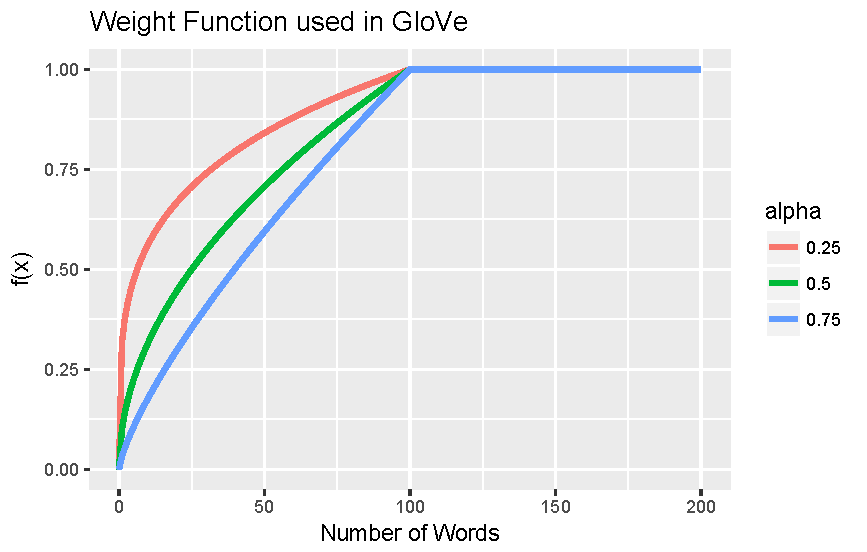
\includegraphics[scale=0.8]{images/weight_fun.pdf} 
\caption[Weight function used in GloVe.]{Illustration of the weight function $f(x)$ for different $\alpha$ values.
        and fixed $x_\mathrm{max} = 100$.}
\label{fig:wf}
\end{figure}

Using this function also introduces two new hyperparameters $\alpha$ and 
$x_\mathrm{max}$. The ordinary way to find good values for $\alpha$ and 
$x_\mathrm{max}$ would be to use a tuning method. The problem now is that the common tuning methods requires that the model can be evaluated. Since we handle an
unsupervised task evaluating isn't straightforward. \\

\textbf{Algorithm used for Fitting} \\

Basically, GloVe uses a gradient descend technique to minimize the objective 
$J$. Nevertheless, using ordinary gradient descend would be way too expensive
in practice. A more appropriate gradient based method is used here called adaptive 
gradient descent (AdaGrad). A short description of the most important properties of 
AdaGrad transferred to text mining are:

\begin{itemize}
  \item
    Individual learning rate in each iteration.

  \item 
    Adaption of the learning rate to the parameters, performing larger updates 
    for infrequent and smaller updates for frequent parameter.

  \item 
    Well-suited for sparse data, improve robustness of (stochastic) gradient 
    descent.
  
  \item 
    For GloVe, infrequent words require much larger updates than frequent ones.
\end{itemize}

For a more detailled explanation see \cite{ruder2016overview}.